\documentclass[12pt]{article}
\title{Towards a `lite' cite legal citation command in non-legal contexts\\[24pt]\normalsize \hfill ---------\hfill\ }
\author{}
\date{}
\usepackage{pdfpages}
\usepackage{xcolor}
\usepackage{fontspec}
\setmainfont{Noto Serif}
\setmonofont{Noto Sans Mono}[Colour=blue]
\newfontface\ftmark{Noto Sans Symbols2}
\newcommand\goodoh{{\large\ftmark 🗸}}
\newcommand\notsogoodoh{{\large\ftmark 🗶}}
\usepackage{fancyhdr} % Needed for customized footer

%\colorbox{white}{\textcolor{white}{\makebox(40,20){XXXXX}}

%\kern-23pt{\raisebox{0.9ex}{\thepage}}

\newcommand\bpn{\textcolor{white}{\raisebox{-3pt}{\rule{40pt}{15pt}}}}

\renewcommand{\headrulewidth}{0.0pt} % Eliminate rule in header
\newcommand{\myfooter}{              % Place the page number 1cm below default position
    \fancyfoot{}
    \fancyfoot[C]{\bpn \rlap{\kern-24pt\thepage}}
}
%\vspace{1cm}

%\fancyfoot[C]{\colorbox{cyan}{\textcolor{white}{\makebox(40,20){XXXXX}}}\\\raisebox{20pt}{\thepage}}


%\parbox[<alignment>][<height>][<inner arrangement>]{<width>}{<text>}
%
%The <height> must be a length which tells LaTeX to build the box as if its vertical dimension were the stated length. The <inner arrangement> must be c, t, b or s (by default the stated or implicit <alignment> is used), that tells how to vertically arrange the text in the available space; s means "spread": all flexible glue available will be used for getting the first line at the top and the last line at the bottom of the available space.



\includepdfset{                      % Setup keys for calls of \includepdf
    pages=-,
%    templatesize={215.9mm}{279.4mm}, % Because the page gets trimmed reset the page size
%    nup=1x1,
    scale=1,
%    clip, 
%    trim=5mm 36.5mm 5mm 20mm,            
%	trim=0mm 0mm 0mm 0mm,        % 
% Trim off the existing page numbers
%    fitpaper=true,
    pagecommand={\myfooter}          % Apply the customized page numbering
}

\pagestyle{fancy}
\fancyhead[L,C,R]{}
%\includepdf[pages=-,addtotoc={
%     1,section,1,First Section Entry,p1,   
%     1,subsection,1,Subsection Entry,p2,
%     2,section,1,Second Section Entry,p3}]
%     {publishing-logo+layout.pdf}    
%
%Parameters for each TOC entry are:
%
%    Page number relative to the first page of the included document. Caveat: with pages={3-10}, the smallest possible number would be 3.
%    Level for the TOC entry
%    Depth of section (1 for section, 2 for subsection, etc.)
%    TOC entry
%    Label for the entry
%
%Apr 17 '11 at 10:10
%Christian Lindig
%
%
%     https://tex.stackexchange.com/questions/15989/toc-entries-and-labels-for-included-pdf-pages

\usepackage[
				bookmarks,
            colorlinks=true,        
            allcolors = black,  
            citecolor=blue,        
]{hyperref}

%=============================================

\newcommand\bef[1]{(\textit{#1})}
\newcommand\cmd[1]{\texttt{\textbackslash #1}}


%=============================================
\begin{document}
\maketitle
\tableofcontents

%\renewcommand*{\HyperDestNameFilter}[1]{\jobname-#1}





%====================================================================
%\section{Numeric style, @article bibentry, custom cite}
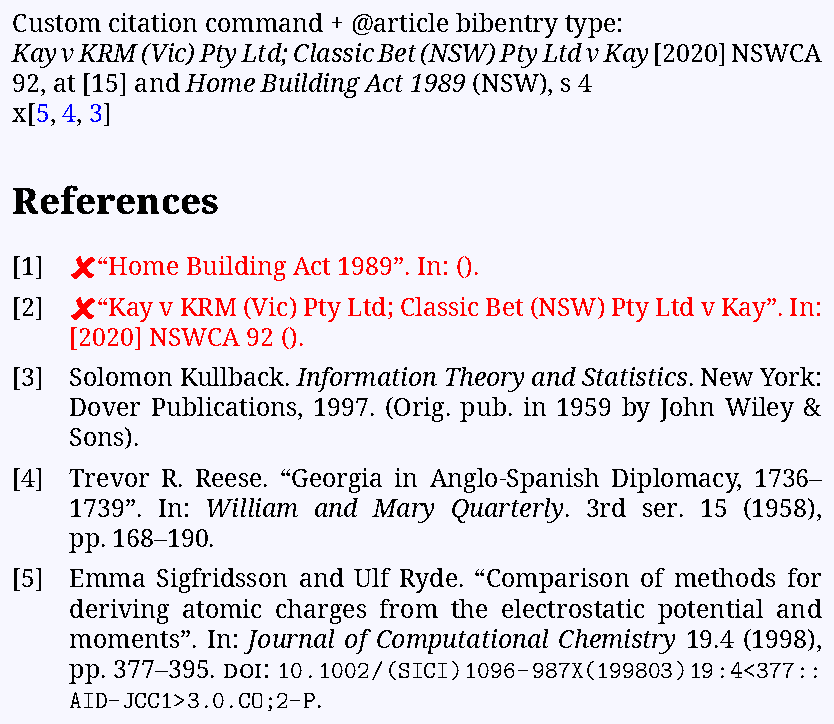
\includepdf[scale=0.8,addtotoc={
     1,section,1,numeric+@article+customcite \notsogoodoh bib,ps12}]{lawcite_example_Dlite.pdf}

\subsection{Custom cite \cmd{legal} citation in numeric style}
\begin{tabular}{lll}
existing   &    bibentry type               & \ttfamily @article \\
existing   &    bibentry fields              & \ttfamily title, number, location, keys \\
existing   &    biblatex style                & \ttfamily numeric \\
custom    &    citation command           & \ttfamily \textbackslash legal \\
existing   &    bib driver                    & (as defined by style) \\
\end{tabular}
\bigskip

The bibentry uses an existing bibentry type and existing fields. Cases and statutes are distinguished via keywords and field sets: both have \bef{title}; cases use \bef{number} to store the case reference, and statutes use \bef{location} to store the jurisdiction. For this scheme, the implicit legal citation style is AGLC3-like. Other fields can be used, as desired.

\begin{verbatim}
@article{sc12,
title = {Kay v KRM (Vic) Pty Ltd},
number = {[2020] NSWCA 92},
keywords={legal,case},
}
T@article{hba,
title = {Home Building Act 1989},
location = {NSW},
keywords={legal,statute},
}
\end{verbatim}

The citation command prints \bef{title} directly, in italics, bypassing the style's formatting for the field, and prints either \bef{number} with \cmd{printfield} or \bef{location} with \cmd{printlist}\footnote{The design purpose of \bef{location} is to store a list of locations of a publisher, e.g., London and New York, although a list can consist of one item as well, e.g. Paris.}, in the existing normal text format, after a space.

\begin{verbatim}
\DeclareCiteCommand{legal}%
{...} 
{%
\mkbibemph{\thefield{title}}%
\iffieldundef{number}{}%
{\addspace\printfield{number}}%case
\iflistundef{location}{}%
{\addspace\mkbibparens{\printlist{location}}}%statute
}%
{...}%
{...}%
\end{verbatim}

The bibliography driver obviously still prints the items as if they were actual articles.

Also, legal citation is inherently an author-title style (with the author being implicit) and not smoothly suited to a numeric style.




%====================================================================
\includepdf[scale=0.8,addtotoc={
     1,section,1,{numeric+@jurisdiction+custombib \goodoh},ps12eb}]{lawcite_example_DliteA_num.pdf}

\subsection{Lite cite \cmd{legal} citation in numeric style}

\begin{tabular}{lll}
existing   &    bibentry type               & \ttfamily @jurisdiction \\
existing   &    bibentry fields              & \ttfamily title, number, location, keys \\
existing   &    biblatex style                & \ttfamily numeric \\
existing   &    citation commands          & (as defined by style) \\
custom    &    bib driver                    & \ttfamily jurisdiction \\
\end{tabular}
\bigskip

Bibentries change over to using the @jurisdiction bibentry type.

\begin{verbatim}
@jurisdiction{sc12,
title = {Kay v KRM (Vic) Pty Ltd},
number = {[2020] NSWCA 92},
keywords={legal,case},
}
@jurisdiction{hba,
title = {Home Building Act 1989},
location = {NSW},
keywords={legal,statute},
}
\end{verbatim}

A custom bibliography driver is defined, using a set of bibmacros, and associated DeclareFieldFormat commands restricted to the @jurisdiction bibentry type, to make things readable and more easily maintainable.

\begin{verbatim}
\DeclareBibliographyDriver{jurisdiction}{%
	\usebibmacro{begentry}
   \usebibmacro{getlegalfull}
	\usebibmacro{finentry}
}
\end{verbatim}

which is built on:

\begin{verbatim}
\DeclareFieldFormat[jurisdiction]{title}{\mkbibemph{#1}}
\DeclareFieldFormat[jurisdiction]{number}{#1}
\DeclareListFormat[jurisdiction]{location}{%
\mkbibparens{#1%
\ifthenelse{\value{listcount}<\value{liststop}}
{\addcomma\space}
{}}}

\newbibmacro{getlegaltitle}{%
\printfield{title}%
}
\newbibmacro{getlegalrefcase}{%
\iffieldundef{number}{}{\printfield{number}}%
}

\newbibmacro{getlegalrefstat}{%
\iflistundef{location}{}{\printlist{location}}%
}

\newbibmacro{getlegalref}{%
\usebibmacro{getlegalrefstat}%
\usebibmacro{getlegalrefcase}%
}

\newbibmacro{getlegalfull}{%
\usebibmacro{getlegaltitle}%
\addspace%
\usebibmacro{getlegalref}%
}
\end{verbatim}


%====================================================================

\includepdf[scale=0.8,addtotoc={
     1,section,1,{author+@article+customcite \notsogoodoh bib},ps12e1}]{lawcite_example_Dlite_auth.pdf}

\subsection{Custom cite \cmd{legal} citation in authortitle style}


\begin{tabular}{lll}
existing   &    bibentry type               & \ttfamily @article \\
existing   &    bibentry fields              & \ttfamily title, number, location, keys \\
existing   &    biblatex style                & \ttfamily authortitle \\
custom    &    citation command           & \cmd{legal} \\
existing   &    bib driver                    & (as defined by style) \\
\end{tabular}
\bigskip






%====================================================================
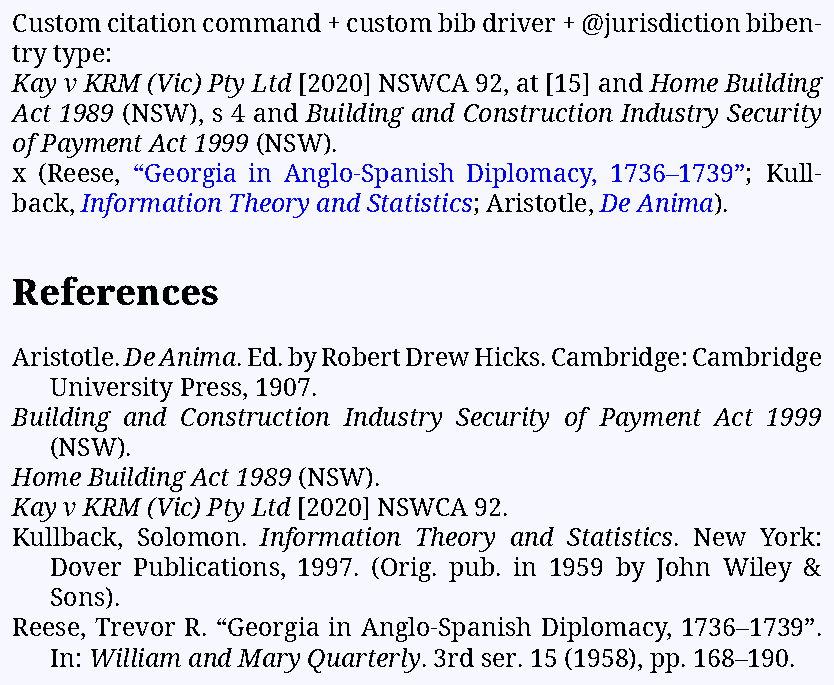
\includepdf[scale=0.8,addtotoc={
     1,section,1,{author+@jurisdiction+customcite/bib \goodoh},ps12e1q}]{lawcite_example_Dlite_autha1.pdf}

\subsection{Lite cite \cmd{legal} citation in authortitle style}


\begin{tabular}{lll}
existing   &    bibentry type               & \ttfamily @jurisdiction \\
existing   &    bibentry fields              & \ttfamily title, number, location, keys \\
existing   &    biblatex style                & \ttfamily authortitle \\
custom    &    citation command           & \cmd{legal} \\
custom    &    bib driver                    & \ttfamily jurisdiction \\
\end{tabular}
\bigskip


%====================================================================
%
\includepdf[scale=0.8,addtotoc={
%     1,section,1,{auth+@jurisdiction},ps12e2}]{lawcite_example_Dlite_jurisa.pdf}





%====================================================================
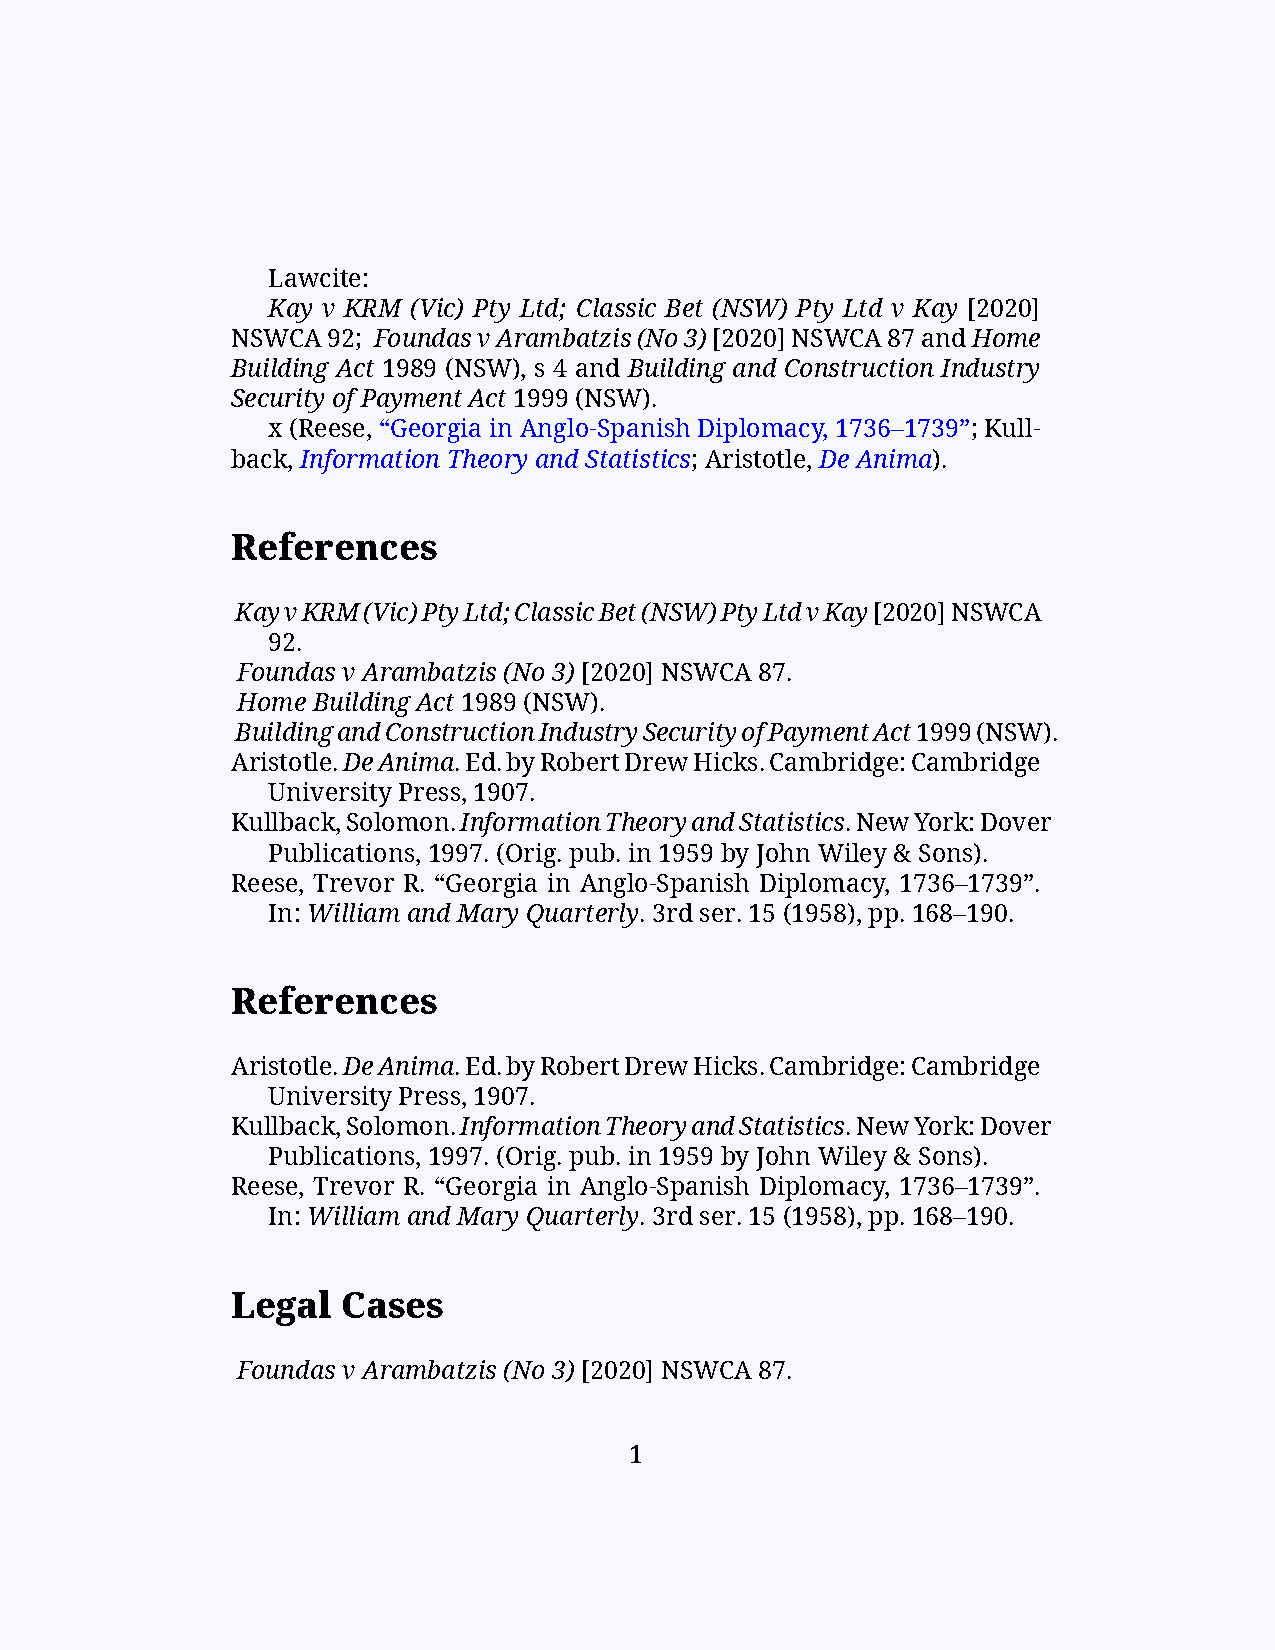
\includepdf[scale=0.8,addtotoc={
     1,section,1,{lawcite+splitbib \goodoh},ps12e3}]{lawcite_example_Dlite_lawcite.pdf}

\subsection{Lawcite style with split legal bibs + no ToC}

If the lawcite biblatex style is installed, and the @case and @statute bibentries have been set up in the bib file, bibliography outputs without a Table of Contents can be produced, emulating the `lite' versions.

In the biblatex package options, switch off lawcite style's Table of Cases\footnote{This is so that the \cmd{sindex} command (from the splitidx package) is not called.}, and, if desired, make the citations inline rather than footnotes for a more authortitle-y look.

\begin{verbatim}
	style=lawcite, 
	set-lawcite-indexing=false,
	lawrefstyle=caseallabove,
	show-statute-jurisdiction=true,
\end{verbatim}

Define some refcontexts for sorting the legal bibliographies (the casesort sorting template will sort the cases, and the statsort sorting template will sort the statutes).

\begin{verbatim}
\DeclareRefcontext{legalcase}{sorting=casesort}
\DeclareRefcontext{legalstat}{sorting=statsort}
%\DeclareRefcontext{legalcasestat}{sorting=casestat}
\end{verbatim}

Print the main, non-legal, bibliography, using the nottype= selectors.

\begin{verbatim}
\printbibliography[nottype=case,nottype=statute]
\end{verbatim}

Apply the case-sorting refcontext, and print the Cases bibliography using the type= selector.
Then apply the statute-sorting refcontext, and print the Legislation bibliography using the type= selector.

\begin{verbatim}
\newrefcontext{legalcase}
\printbibliography[type=case,title=Legal Cases]
\newrefcontext{legalstat}
\printbibliography[type=statute,title=Legislation]
\end{verbatim}



%====================================================================
\includepdf[scale=0.8,addtotoc={
     1,section,1,{lawcite+combbib \goodoh},ps12e4}]{lawcite_example_Dlite_lawcitea1.pdf}

\subsection{Lawcite style with combined legal bib + no ToC}

To print cases and statutes together in a separate bibliography, define a refcontext that will sort on both simultaneously (using the casestat sorting template).

\begin{verbatim}
\DeclareRefcontext{legalcasestat}{sorting=casestat}
\end{verbatim}

Define a filter that will retrieve both entry types.

\begin{verbatim}
\defbibfilter{legal}{type=case or type=statute}
\end{verbatim}

Apply the refcontext for the sorting and print the legal bibliography using the filter= selector,

\begin{verbatim}
\newrefcontext{legalcasestat}
\printbibliography[filter=legal,title=Legal]
\end{verbatim}



%====================================================================

\includepdf[scale=0.8,addtotoc={
     1,section,1,{lawcite+subbibs \goodoh},ps12e4}]{lawcite_example_Dlite_lawcitea2.pdf}


\subsection{Lawcite style with legal subbibs + no ToC}

To print cases and statutes as separate subbibligraphies within a legal bibliography, define a bibheading for the overall bibliography (section-level if using article class; chapter-level if using book class).


\begin{verbatim}
\defbibheading{lm}{%
\section*{Legal Material}}
\end{verbatim}

Print the bib heading.

\begin{verbatim}
\printbibheading[heading=lm]
\end{verbatim}

Apply the refcontext for sorting cases, and print the case subbibliography using the type= selector, and setting the subbib title to subbibliography format using heading=subbibliography.

\begin{verbatim}
\newrefcontext{legalcase}
\printbibliography[type=case,
title=Cases,
heading=subbibliography]
\end{verbatim}

Similarly for statutes.

\begin{verbatim}
\newrefcontext{legalstat}
\printbibliography[type=statute,
title=Legislation,
heading=subbibliography]
\end{verbatim}




%====================================================================
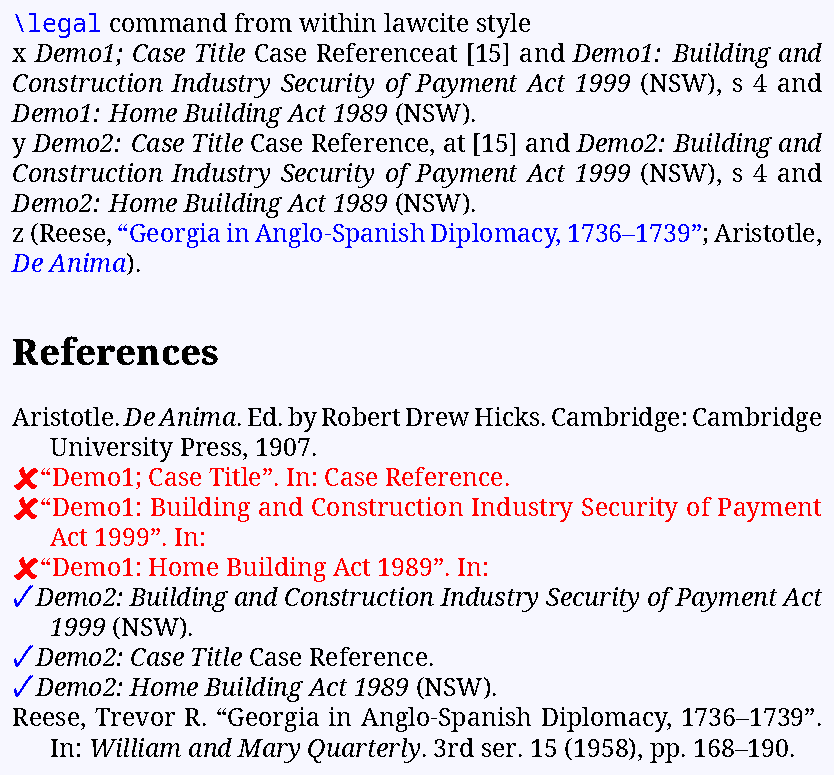
\includepdf[scale=0.8,addtotoc={
     1,section,1,{lawcite+\cmd{legal} \goodoh},ps12e5}]{lawcite_example_Dlite_demo.pdf}


\subsection{Lawcite style with \cmd{legal} + no ToC}
The \cmd{legal} `lite' cite citation command, at (x) and (y), and the 
`lite' \bef{jurisdiction} bib driver, at (Demo 2), are now available as part the lawcite biblatex style, without needing to be coded up in the preamble.
\bigskip

\noindent (x) is an @article bibentry type.

\noindent (y) is a @jurisdiction bibentry type.
\bigskip
\bigskip

\hfill ---------\hfill\ 

\bigskip

Summary: Litecites

%\begin{quotation}
\begin{itemize}
\item If only citations are needed:
	\begin{itemize}
	\item Use the \cmd{legal} citation command
	\item on any bibentry types, which have
		\begin{itemize}
		\item either: \bef{title} and \bef{number} fields -- for cases
		\item or: \bef{title} and \bef{location} fields -- for statutes
		\end{itemize}
	\end{itemize}
\item If a bibliographic entry is also needed:
	\begin{itemize}
	\item Use the \cmd{legal} citation command
	\item on the @jurisdiction bibentry type, which should have the \bef{title} field and, optionally,
		\begin{itemize}
		\item either:  a \bef{number} field for the case reference(s) -- for cases
		\item or: a \bef{location} field for the jurisdiction (or year, if it is not part of the title) -- for statutes.
		\end{itemize}
		\item Sorting within the bibliography is taken care of by numeric or authortitle styles using the \bef{title} field or, alternatively,
		\item a sorting template may be defined in the preamble (for example, sorting legislation chronologically).
		\item And, keywords in the bibentry may be used for filtering into separate bibliographies or subbibliographies.
	\end{itemize}
\end{itemize}
%\end{quotation}



\bigskip
\bigskip
\hfill --oooOooo--\hfill\ 


\end{document}





